\chapter{Tutorium 07 - 04.12.2025}
\section{Task 1}
\begin{equation*}
    d(v_i, v_j) = min(2\cdot |i-j|, \mid (1+\delta)+(1+\delta)) = min (2\cdot |i-j|, \mid 2+2\cdot\delta)
\end{equation*}
\begin{mybox}[title=Terminal nodes]
Terminal nodes in a DNA grid graph are all given sequences and the other nodes (internal nodes, non-terminal nodes) are all possible sequences. 
\end{mybox}
\begin{figure}[H]
    \centering
    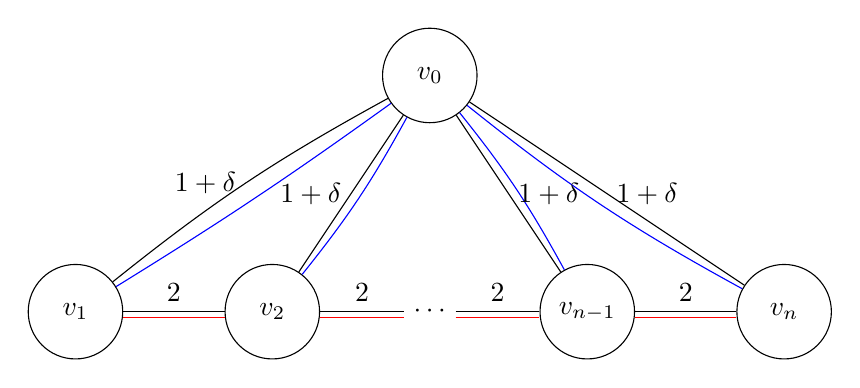
\begin{tikzpicture}
   \node [circle, draw, minimum size=1.2cm] (v0) at (0,1) {$v_0$}; 
   \node (dots) at (0,-2) {$\cdots$}; 
   \node [circle, draw, minimum size=1.2cm] (v1) at (-4.5,-2) {$v_1$};
   \node [circle, draw,  minimum size=1.2cm] (v2) at (-2,-2) {$v_2$};
   \node [circle, draw,  minimum size=1.2cm] (vn1) at (2,-2) {$v_{n-1}$};
   \node [circle, draw,  minimum size=1.2cm] (vn) at (4.5,-2) {$v_{n}$};
   
   \path[blue] (v0) edge[bend left=2] (v1) 
                        (v0) edge[bend left=5] (v2)
                        (v0) edge[bend left=5] (vn1)
                        (v0) edge[bend right=5] (vn);
                    
    \path[red, transform canvas={yshift=-2pt}]  
                (dots) edge (vn1)
                (vn1) edge (vn)
                (v1) edge (v2)
                (v2) edge  (dots);
    
   \path[black] (v0) edge[bend right=5]  node[left]  {$1+\delta$} (v1) 
                (v0) edge node[left]  {$1+\delta$} (v2)
                (v0) edge node[right]  {$1+\delta$} (vn1)
                (v0) edge node[right]  {$1+\delta$} (vn)
                (dots) edge node[above]  {$2$} (vn1)
                (vn1) edge node[above]  {$2$} (vn)
                (v1) edge node[above]  {$2$} (v2)
                (v2) edge node[above]  {$2$} (dots);
    
            
\end{tikzpicture}
    \caption{\textcolor{red}{T} und \textcolor{blue}{R}.}
    \label{fig:my_label}
\end{figure}
\begin{align*}
    C(T) &= 2 \cdot (n-1) \\
    C(R) &= n \cdot (1+\delta)
\end{align*}
Keine Ahnung warum man das jetzt so rechnet (TODO), aber:
\begin{equation*}
    \frac{C(T)}{C(R)} = \frac{2\cdot(n-1)}{n\cdot(1+\delta)} = \frac{2\cdot (1-\frac{1}{n})}{1+\delta}
\end{equation*}
Es soll für beliebig große Datensets funktionieren, also lassen wir zum Lösen $n$ gegen unendlich laufen und da wir $\delta$ frei wählen können, lassen wir es gegen Null laufen: 
\[
\frac{2\cdot (1-\frac{1}{''\infty''})}{1+0} = \frac{2\cdot (1-0)}{1} = \frac{2\cdot 1}{1} = 2
\]
\section{Task 2 - Additive Metric, Ultrametric}
\begin{mechanism}[title=Frage]
\textbf{F:} Wenn wir gezeigt haben eine Metrik ist ultrametrisch, müssen wir auch noch zeigen sie ist additiv? (Beliebte Klausurfrage von Roland) \\
\textbf{A:} Nein! Additiv bedeutet sozusagen es ist ein Baum und ultrametrisch bedeutet es ist ein Baum, bei dem die Wurzel-Blatt-Distanz immer gleich ist.  \\
$\Rightarrow$ ultrametrisch impliziert immer additiv
\end{mechanism}
Advice for exam: do not memorize the inequality formula, remember the graphs (7.2, 7.3)
\subsection{(a) Show that matrix i) describes an ultrametric}
Three point condition - We have to do all pairs! \\
\textbf{Anmerkung:} 
\begin{center}
    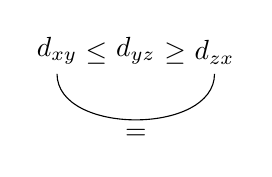
\begin{tikzpicture}
  \coordinate [label=$d_{xy}$]  (A) at (0,0);
  \coordinate [label=$d_{yz}$]  (B) at (1,0);
  \coordinate [label=$d_{zx}$]  (C) at (2,0);
  \coordinate [label=$\leq$] (Z)  at (0.5,0);
  \coordinate [label=$\geq$] (Y)  at (1.5,0);
   \draw (A) to [out=-90,in=-90] node [sloped,below] {$=$} (C);
\end{tikzpicture}
\end{center}


\subsection{(b) Show that matrix ii) describes an additive metric, but not an ultrametric}
Four point condition 


